% $Header: /cvsroot/latex-beamer/latex-beamer/solutions/conference-talks/conference-ornate-20min.en.tex,v 1.6 %2004/10/07 20:53:08 tantau Exp $
\documentclass[xcolor=table,spanish,9pt]{beamer}

% This file is a solution template for:

% - Talk at a conference/colloquium.
% - Talk length is about 20min.
% - Style is ornate.



% Copyright 2004 by Till Tantau <tantau@users.sourceforge.net>.
%
% In principle, this file can be redistributed and/or modified under
% the terms of the GNU Public License, version 2.
%
% However, this file is supposed to be a template to be modified
% for your own needs. For this reason, if you use this file as a
% template and not specifically distribute it as part of a another
% package/program, I grant the extra permission to freely copy and
% modify this file as you see fit and even to delete this copyright
% notice. 


\mode<presentation>
{
  \usetheme{Warsaw}
  % or ...

  %\setbeamercovered{transparent}
  % or whatever (possibly just delete it)
}

\usepackage{babel} %entiende español y el resto de los lenguajes, sirve para las secciones
\usepackage{ucs}
\usepackage[utf8x]{inputenc} % acentos y eñes
\usepackage[T1]{fontenc}
\usepackage{amsmath}
\usepackage{graphics} % lo necesita el listings
\usepackage{graphicx}
\usepackage{listings} % con eso le doy formato al codigo fuente
\usepackage{wrapfig} % para meter figuras entre el texto
\usepackage{tikz}
\usepackage{multirow}
\usetikzlibrary{arrows,automata,shapes}
\usetikzlibrary{fit}
\usepackage{listings}
\usepackage[labelformat=empty]{caption}

\newcommand\Myast{\raisebox{0.3pt}{*}}

\lstset{language=C++,
tabsize=4,
basicstyle= \tiny, %\footnotesize, 	%\small,
morekeywords=[3]{requires,normal_behavior,decreases,modifies,ensures,invariant,
loop_invariant,model,modifiable,pure, \result, \nothing, \exists, \forall,
\old,set,ghost, signals, exceptional_behavior, also, showspaces=false, showstringspaces=false},
keywordstyle=[3]\bfseries\itshape,
moredelim=**[s][commentstyle]{/*@}{@*/},
moredelim=**[l][commentstyle]{//@},
showspaces=false,
showstringspaces=false,
showtabs=false,
escapeinside=||
}


%\usepackage[english]{babel} - templante
% or whatever

%\usepackage[latin1]{inputenc} -template
% or whatever

\usepackage{times}
%\usepackage[T1]{fontenc} -template
% Or whatever. Note that the encoding and the font should match. If T1
% does not look nice, try deleting the line with the fontenc.

\title[Punteros, Referencias y Manejo de Memoria en C++]{Punteros, Referencias y Manejo de Memoria en C++}   %[Short Paper Title] % (optional, use only with long paper titles)


%\subtitle{Include Only If Paper Has a Subtitle}

\author[Mat\'ias L. Marenchino] % (optional, use only with lots of authors)
{Mat\'ias L. Marenchino}%{~Author \and S.~Another\inst{2}}

% - Give the names in the same order as the appear in the paper.
% - Use the \inst{?} command only if the authors have different
%   affiliation.

%\institute[Universities of Somewhere and Elsewhere] % (optional, but mostly needed)
%{
%  \inst{1}%
%  Department of Computer Science\\
%  University of Somewhere
%  \and
%  \inst{2}%
%  Department of Theoretical Philosophy\\
%  University of Elsewhere}
% - Use the \inst command only if there are several affiliations.
% - Keep it simple, no one is interested in your street address.

\date % (optional, should be abbreviation of conference name)
{28 de junio de 2012 \\ \mbox{} \\ Ascentio Technologies S.A.}
% - Either use conference name or its abbreviation.
% - Not really informative to the audience, more for people (including
%   yourself) who are reading the slides online



% If you have a file called "university-logo-filename.xxx", where xxx
% is a graphic format that can be processed by latex or pdflatex,
% resp., then you can add a logo as follows:

\pgfdeclareimage[height=0.5cm]{ascentio-logo}{./figures/logo_ascentio.png}
\logo{\pgfuseimage{ascentio-logo}}


% Delete this, if you do not want the table of contents to pop up at
% the beginning of each subsection:
\AtBeginSubsection[]
{
  \begin{frame}<beamer>
    \frametitle{Outline}
    \tableofcontents[currentsection,currentsubsection]
  \end{frame}
}


% If you wish to uncover everything in a step-wise fashion, uncomment
% the following command: 

%\beamerdefaultoverlayspecification{<+->}


\begin{document}

\begin{frame}
  \titlepage
\end{frame}

\begin{frame}[allowframebreaks]
  \frametitle{Tabla de Contenidos}
  \tableofcontents
  % You might wish to add the option [pausesections]
\end{frame}

% Structuring a talk is a difficult task and the following structure
% may not be suitable. Here are some rules that apply for this
% solution: 

% - Exactly two or three sections (other than the summary).
% - At *most* three subsections per section.
% - Talk about 30s to 2min per frame. So there should be between about
%   15 and 30 frames, all told.

% - A conference audience is likely to know very little of what you
%   are going to talk about. So *simplify*!
% - In a 20min talk, getting the main ideas across is hard
%   enough. Leave out details, even if it means being less precise than
%   you think necessary.
% - If you omit details that are vital to the proof/implementation,
%   just say so once. Everybody will be happy with that.

\section{Punteros}


% http://www-control.eng.cam.ac.uk/~pcr20/www.cppreference.com/keywords.html
% \begin{frame}[fragile]
% \begin{tabular}{|c|l|}
% \hline
% asm &		insert an assembly instruction \\ \hline
% auto&		declare a local variable \\ \hline 
% bool&		declare a boolean variable \\ \hline 
% break&		break out of a loop \\ \hline 
% case&		part of a switch statement \\ \hline 
% catch&		handles thrown exceptions \\ \hline 
% char&		declare a character variable \\ \hline 
% class&		declare a class \\ \hline 
% const&		declare immutable data \\ \hline 
% const\_cast&	cast from const variables \\ \hline 
% continue&	bypass iterations of a loop \\ \hline 
% default&	default handler in a case statement \\ \hline 
% delete&		free memory \\ \hline 
% do&		looping construct \\ \hline 
% double&		declare a double precision floating-point variable \\ \hline 
% dynamic\_cast&	perform runtime casts \\ \hline 
% else&		alternate case for an if statement \\ \hline 
% enum&		create enumeration types \\ \hline 
% \end{tabular}
% \end{frame}
% \begin{frame}[fragile]
% \begin{tabular}{|c|l|}
% \hline
% explicit&	only use constructors when they exactly match \\ \hline 
% extern&		tell the compiler about variables defined elsewhere \\ \hline 
% false&		the boolean value of false \\ \hline 
% float&		declare a floating-point variable \\ \hline 
% for&		looping construct \\ \hline 
% friend&		grant non-member function access to private data \\ \hline 
% goto&		jump to a different part of the program \\ \hline 
% if&		execute code based off of the result of a test \\ \hline 
% inline&		expand a call to a function rather than calling that function \\ \hline 
% int&		declare a integer variable \\ \hline 
% long&		declare a long integer variable \\ \hline 
% mutable&	override a const variable \\ \hline 
% namespace&	partition the global namespace by defining a scope \\ \hline 
% new&		allocate dynamic memory for a new variable \\ \hline 
% operator&	create overloaded operator functions \\ \hline 
% private&	declare private members of a class \\ \hline 
% protected&	declare protected members of a class \\ \hline 
% \end{tabular}
% \end{frame}
% \begin{frame}[fragile]
% \begin{tabular}{|c|l|}
% \hline
% public&		declare public members of a class \\ \hline 
% register&	request that a variable be optimized for speed \\ \hline 
% reinterpret\_cast&	change the type of a variable \\ \hline 
% return&		return from a function \\ \hline 
% short&		declare a short integer variable \\ \hline 
% signed&		modify variable type declarations \\ \hline 
% sizeof&		return the size of a variable or type \\ \hline 
% static&		create permanent storage for a variable \\ \hline 
% static\_cast&	perform a nonpolymorphic cast \\ \hline 
% struct&		create a new structure \\ \hline 
% switch&		execute code based off of different possible values \\ \hline 
% template&	create generic functions \\ \hline 
% this&		a pointer to the current object \\ \hline 
% throw&		throws an exception \\ \hline 
% true&		the boolean value of true \\ \hline 
% try&		execute code that can throw an exception \\ \hline 
% typedef&	create a new type name from an existing type \\ \hline 
% \end{tabular}
% \end{frame}
% \begin{frame}[fragile]
% \begin{tabular}{|c|l|}
% \hline
% typeid&		describes an object \\ \hline 
% typename&	declare a class or undefined type \\ \hline 
% union&		a structure that assigns multiple variables to the same memory \\ \hline 
% unsigned&	declare an unsigned integer variable \\ \hline 
% using&		used to import a namespace \\ \hline 
% virtual&	create a function that can be overridden by a derived class \\ \hline 
% void&		declare functions or data with no associated data type \\ \hline 
% volatile&	warn compiler about variables that can be modified unexpectedly \\ \hline 
% wchar\_t&	declare a wide-character variable \\ \hline 
% while&		looping mechanism \\ \hline 
% \end{tabular}
% \end{frame}


\subsection{Qué son}

\begin{frame}[fragile]
  \begin{alertblock}{Definición}
    Un puntero es una variable que almacena una dirección de memoria.
  \end{alertblock}
  \begin{block}{Qué es una dirección de memoria}
    \begin{itemize}
      \item Las variables son ubicadas en una ubicación única dentro de la memoria de la computadora. Esta única ubicación tiene asociada una única dirección, 
	    la dirección de memoria.
      \item En general, las variables contienen valores como el número 5 o la palabra ``hola'' y éstos valores son almacenados en una ubicación específica en la memoria.
      \item Pero los punteros son diferentes porque almacenan direcciones de memoria (y tienen la habilidad de apuntar -puntero- mediante el uso de tal dirección).
    \end{itemize}
  \end{block}
\end{frame}


\subsection{Operadores}

\begin{frame}[fragile]
  \begin{block}{$*$}
    Permite definir un puntero:
    \begin{lstlisting}
      int *p;
      int *q = 0;
      int *r = NULL;
      void *s;
    \end{lstlisting}
  \end{block}
  \begin{figure}
    \centering
    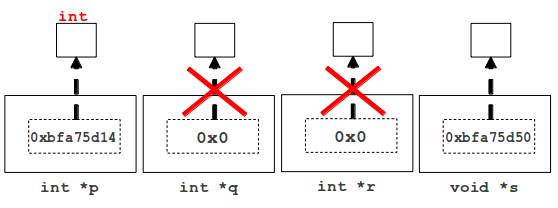
\includegraphics[width=6cm,height=2cm,keepaspectratio=true,clip=true]
    {./figures/pointers_definitions.png}\\
  \end{figure}
\end{frame}

\begin{frame}[fragile]
  \begin{block}{Reference operator \&}
    \begin{lstlisting}
      int n = 25;
      int *p = &n;
    \end{lstlisting}
  \end{block}
  \begin{figure}
    \centering
    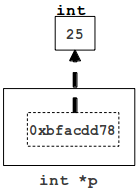
\includegraphics[width=6cm,height=2cm,keepaspectratio=true,clip=true]
    {./figures/pointer_to_int.png}\\
  \end{figure}
\end{frame}

\begin{frame}[fragile]
  \begin{block}{Dereference operator *}
    \begin{lstlisting}
      int n = 25;
      int *p = &n;
      int m = *p;
    \end{lstlisting}
  \end{block}
  \begin{figure}
    \centering
    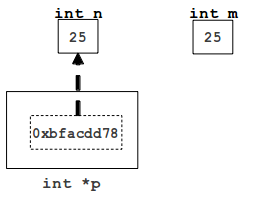
\includegraphics[width=6cm,height=2cm,keepaspectratio=true,clip=true]
    {./figures/dereference.png}\\
  \end{figure}
\end{frame}

\begin{frame}[fragile]
  \begin{block}{Identidad}
    p == \&*p == *\&p
  \end{block}
  \begin{block}{Copia de punteros}
    \begin{lstlisting}
      int n = 25;
      int *p = &n;
      int *q = p;
    \end{lstlisting}
  \end{block}
  \begin{figure}
    \centering
    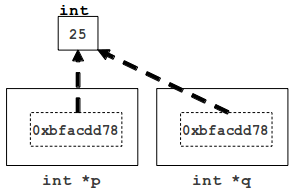
\includegraphics[width=6cm,height=2cm,keepaspectratio=true,clip=true]
    {./figures/copy_pointers.png}\\
  \end{figure}
\end{frame}


\subsection{Arreglos}

\begin{frame}[fragile]
  \begin{block}{Definición}
    Un arreglo en C++ es un conjunto de datos que se alamacenan en memoria de manera contigua con el mismo nombre.
  \end{block}
  \begin{block}{Ejemplo}
    \begin{lstlisting}
      int firstarray [] = {5, 10};
      int secondarray [3] = {2, 4, 6};
      int lastarray [3];
      int *p = firstarray;
    \end{lstlisting}
  \end{block}
  \begin{figure}
    \centering
    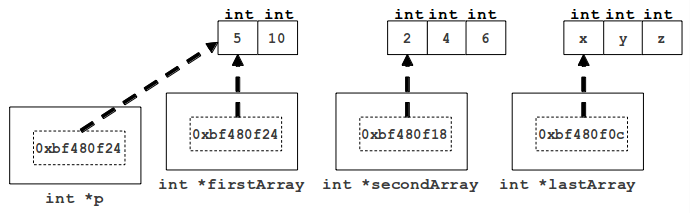
\includegraphics[width=6cm,height=2cm,keepaspectratio=true,clip=true]
    {./figures/arrays.png}\\
  \end{figure}
  \begin{alertblock}{Qué pasa si?}
    \begin{lstlisting}
      lastarray = secondarray;
    \end{lstlisting}
  \end{alertblock}
\end{frame}


\subsection{Operaciones sobre arreglos}

\begin{frame}[fragile]
  \begin{block}{Acceso a elementos}
    El acceso a un elemento de un arreglo se hace de la siguiente manera:
    \begin{lstlisting}
      name [index];
    \end{lstlisting}
    El tipo de tal expresión será el mismo al cual apunta la variable ``name''.
  \end{block}
  \begin{block}{Aritmética sobre punteros}
    \begin{lstlisting}
      int array [3] = {5, 10, 15};
      int *p = array;
      int *q = p + 1;                                                             p++;
      int *r = q - 1;
    \end{lstlisting}
    \begin{columns}
      \begin{column}{.65\linewidth}
	\begin{figure}
	  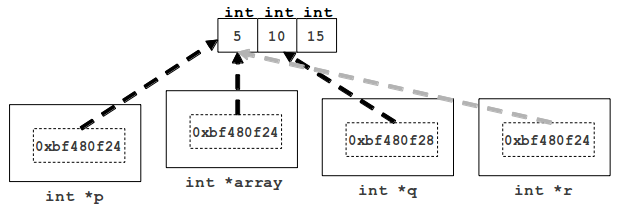
\includegraphics[width=6cm,keepaspectratio=true,clip=true]
	  {./figures/pointers_arithmetics.png}\\
	\end{figure}
      \end{column}
      \begin{column}{.35\linewidth}
	\begin{figure}
	  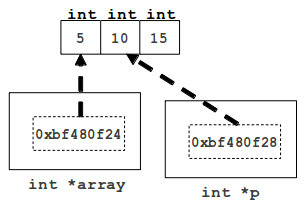
\includegraphics[width=3cm,keepaspectratio=true,clip=true]
	  {./figures/pointers_increase.png}\\
	\end{figure}
      \end{column}
    \end{columns}
  \end{block}
\end{frame}


\subsection{Arreglos multidimensionales}

\begin{frame}[fragile]
  \begin{block}{Qué son}
    Pueden verse como arreglos de arreglos. Por ejemplo, en el caso de 2 dimensiones, son Matrices.
  \end{block}
  \begin{block}{Ejemplo}
    \begin{lstlisting}
      int matrix [3][2]; 
    \end{lstlisting}
    \begin{figure}
      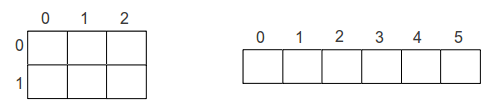
\includegraphics[width=6cm,keepaspectratio=true,clip=true]
      {./figures/matrix.png}\\
    \end{figure}
  \end{block}
\end{frame}


\subsection{Punteros constantes}

\begin{frame}[fragile]
  \begin{block}{Puntero a constante}
    \begin{lstlisting}
      const int *p = ....;
    \end{lstlisting}
  \end{block}
  \begin{block}{Puntero constante}
    \begin{lstlisting}
      int * const p; 
    \end{lstlisting}
  \end{block}
  \begin{block}{Puntero constante a constante}
    \begin{lstlisting}
      const int * const p = ....; 
    \end{lstlisting}
  \end{block}
\end{frame}


\subsection{Tamaño de punteros}

\begin{frame}[fragile]
  Ejemplos:
  \begin{lstlisting}
    int i = 10;
    int *p = &i;
    int array [3] = {1,2,3};
    float secondArray [5];
    int *q = array;
  \end{lstlisting}
  \begin{block}{Tamaños}
    sizeof(i) = 4\\
    sizeof(p) = 4\\
    sizeof(array) = 12\\
    sizeof(secondArray) = 40\\
    sizeof(q) = 4\\
  \end{block}
\end{frame}



\section{Referencias}

\subsection{Qué son}

\begin{frame}[fragile]
  \begin{alertblock}{Definición}
    Una referencia es un nombre alternativo para un objeto. Es como un puntero constante que se de-referencia automáticamente. 
    Es una especie de alias o ``alter ego'' del objeto al que se refiere.
  \end{alertblock}
  \begin{block}{\&}
    \begin{lstlisting}
      int i = 10;
      int &r = i;
    \end{lstlisting}
    Todo aquello que le haga a $r$, se verá reflejado en $i$ (y viceversa).
  \end{block}
\end{frame}


\subsection{Implementación}

\begin{frame}[fragile]
  \begin{columns}
    \begin{column}{.3\linewidth}
      \begin{center}
	Punteros
	\begin{lstlisting}
  int i = 4;
  int|\Myast| pi = &i;
	\end{lstlisting}
      \end{center}
    \end{column}
    \begin{column}{.5\linewidth}
      \begin{center}
	Referencias
	\begin{lstlisting}
  int i = 4;
  int& ri = i;
	\end{lstlisting}
      \end{center}
    \end{column}
  \end{columns}  
  \begin{figure}
    \centering
    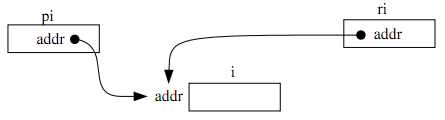
\includegraphics[width=6cm,height=2cm,keepaspectratio=true,clip=true]
    {./figures/pointers_references.png}\\
  \end{figure}
  {\bf Acceso}
  \begin{columns}
    \begin{column}{.3\linewidth}
      \begin{center}
	\begin{lstlisting}
  cout << |\Myast|pi << endl;
	\end{lstlisting}
      \end{center}
    \end{column}
    \begin{column}{.5\linewidth}
      \begin{center}
	\begin{lstlisting}
  cout << ri << endl;
	\end{lstlisting}
      \end{center}
    \end{column}
  \end{columns}
  {\bf Manejo de memoria}
  \begin{columns}
    \begin{column}{.3\linewidth}
      \begin{center}
	\begin{lstlisting}
  pi++;
	\end{lstlisting}
      \end{center}
    \end{column}
    \begin{column}{.5\linewidth}
      \begin{center}
	\begin{lstlisting}
  //imposible, la referencia es constante
	\end{lstlisting}
      \end{center}
    \end{column}
  \end{columns} 
\end{frame}

\begin{frame}[fragile]
\frametitle{Ejemplos en la práctica}
  \begin{lstlisting}
    int i = 10;
    int &r = i;
    r = 20;               // i = 20, j = UND, r = 20
    int j = 34;
    r = j;                // i = 34, j = 34,  r = 34
    j++;                  // i = 34, j = 35,  r = 34
  \end{lstlisting}
  ========================================================
  \begin{lstlisting}
    int *p = new int(3);          // *p = 3, r = UND
    int &r = *p;                  // *p = 3, r = 3
    r++;                          // *p = 4, r = 4
    p++;                          // SOAB
    ...
  \end{lstlisting}
  ========================================================
  \begin{columns}
    \begin{column}{.33\linewidth}
      \begin{lstlisting}
	void swap(int a, int b)
	{
	  int tmp = a;
	  a = b;
	  b = tmp;
	}
	...
	int main (void)
	{
	  int x = 3, y = 7;
	  swap(x, y);
	  // x = 3 & y = 7
	  ...
      \end{lstlisting}
    \end{column}
    \begin{column}{.33\linewidth}
      \begin{lstlisting}
	void swap(int *a, int *b)
	{
	  int tmp = *a;
	  *a = *b;
	  *b = tmp;
	}
	...
	int main (void)
	{
	  int x = 3, y = 7;
	  swap(&x, &y);
	  // x = 7 & y = 3
	  ...
      \end{lstlisting}
    \end{column}
    \begin{column}{.33\linewidth}
      \begin{lstlisting}
	void swap(int &a, int &b)
	{
	  int tmp = a;
	  a = b;
	  b = tmp;
	}
	...
	int main (void)
	{
	  int x = 3, y = 7;
	  swap(x, y);
	  // x = 7 & y = 3
	  ...
      \end{lstlisting}
    \end{column}
  \end{columns}
\end{frame}


\section{Alocación de memoria}

\subsection{Uso}

\begin{frame}[fragile]
  \begin{alertblock}{new y delete}
    Los operadores new y delete constituyen la manera para hacer asignación dinámica de memoria y lirerarla.
    Son una evolución de los operadores malloc y free del lenguaje C.
  \end{alertblock}
  \begin{block}{Uso}
    Se usan de a pares: new y delete  o  new [] y delete [].\\
    Cada vez que se solicita memoria mediante una llamada a new, se debe matener la referencia a esa porción de memoria para después liberarla con el operador 
    delete.
  \end{block}
\end{frame}


\subsection{Ejemplo}

\begin{frame}[fragile]
  \begin{block}{new y delete}
    \begin{lstlisting}
      int *p;
      p = new int;
      *p = 2;
      ...;
      delete p;
    \end{lstlisting}
    \begin{figure}
      \centering
      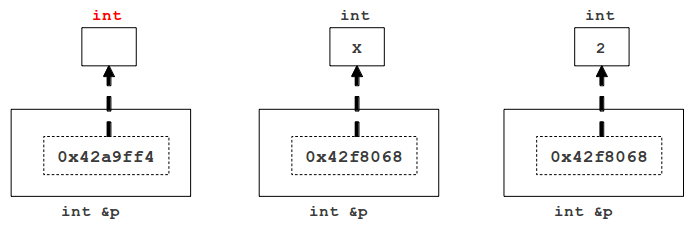
\includegraphics[width=6cm,height=2cm,keepaspectratio=true,clip=true]
      {./figures/new_operator.png}\\
    \end{figure}
  \end{block}
\end{frame}



\begin{frame}[fragile]
  \begin{block}{new [] y delete []}
    \begin{lstlisting}
      int *p;
      p = new int [2];
      p[0] = 2;
      p[1] = 3;
      ...;
      delete [] p;
    \end{lstlisting}
    \begin{figure}
      \centering
      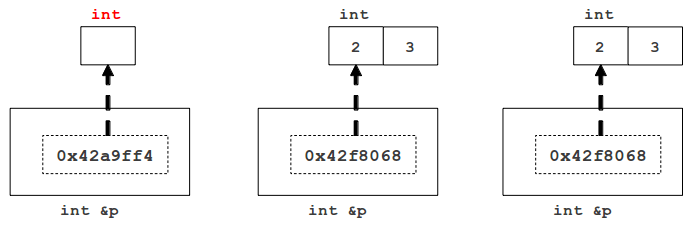
\includegraphics[width=6cm,height=2cm,keepaspectratio=true,clip=true]
      {./figures/new_array.png}\\
    \end{figure}
\end{block}
\end{frame}


% \section{Coding Style}
% 
% \subsection{C++ Programming Style}
% 
% \begin{frame}[fragile]
%   \begin{block}{Convenciones}
%     \begin{itemize}
%       \item Nombres de tipos en mixed case con inicial mayúscula: Matrix
%       \item Nombres de variables en mixed case con inicial minúscula: rotationMatrix
%       \item Nombres de constantes en mayúscula con ``\_'' para separar palabras: MAX\_ITERATIONS
%       \item Nombres de métodos verbos en mixed case con inicial minúscula: sortNumbers()
%       \item Nombres de namespaces en minúscula: matrices::
%       \item Nombres de templates en una letra sola en mayúscula: template <typename T>
%       \item En los acrónimos no se usan mayúsculas: openDvdPlayer()
%       \item Variables globales se llaman con el operador ::
%       \item Atributos privados de métodos con ``\_'' como sufijo: nRows\_
%       \item http://geosoft.no/development/cppstyle.html
%     \end{itemize}
%   \end{block}
% \end{frame}
% 
% 
% 
% \section{Buenas Prácticas}
% 
% \subsection{Ejemplo de librería a implementar}
% 
% \begin{frame}[fragile]
%   \frametitle{Librería de Matrices con elementos flotantes}
%    \begin{figure}
%      \centering
%      \includegraphics[width=8cm,height=8cm,keepaspectratio=true,clip=true]
%      {./figures/class_diagram.png}\\
%    \end{figure}
% \end{frame}
% 
% 
% \subsection{Items}
% 
% \begin{frame}[fragile]
%   \frametitle{Evitar el uso de {\bf \#define}}
%   \tiny
%   \begin{lstlisting}
% #define MAX(a,b) (a < b) ?  b : a
% 
% class MultidimensionalArray
% {
% public:
%   MultidimensionalArray (int dimension, ...);
%   MultidimensionalArray (double|\Myast| array, int dimension, ...);
%   ~MultidimensionalArray();
%   double max();
% ...        
%   \end{lstlisting}
%   \begin{columns}
%     \begin{column}{.45\linewidth}\onslide<2->
%       \begin{block}{Uso 1}
% 	\begin{lstlisting}
% double x = 2.6;
% double y = 1.0;
% double max = MAX(x,++y);
% 	\end{lstlisting}
%       \end{block}
%       \onslide<4->
%       \begin{block}{Uso 2}
% 	\begin{lstlisting}
% double x = 1.0;
% double y = 2.6;
% double max = MAX(x,++y);
% 	\end{lstlisting}
%       \end{block}
%     \end{column}
%     \begin{column}{.55\linewidth}\onslide<3->
%       \begin{alertblock}{Resultado}
% 	\begin{lstlisting}
% max = 2.6;
% 	\end{lstlisting}
%       \end{alertblock}
%       \onslide<5->
%       \begin{alertblock}{Resultado}
% 	\begin{lstlisting}
% max = 4.6;
% 	\end{lstlisting}
%       \end{alertblock}
%     \end{column}
%   \end{columns}
% \end{frame}
% 
% 
% \begin{frame}[fragile]
%   \frametitle{Evitar el uso de {\bf \#define}}
%   \tiny
%   \begin{lstlisting}
% #define PI 3.141592
% 
% RotationMatrix::RotationMatrix (double angle, char axis, bool isRadian) : Matrix(3,3)
% {
%     double radians = angle;
%     if (!isRadian){
%         radians = angle |\Myast| PI / 180.0;
%     }
% ...        
%   \end{lstlisting}
%    \begin{figure}
%      \centering
%      \includegraphics[height=4cm,keepaspectratio=true,clip=true]
%      {./figures/debugging_macros.png}\\
%    \end{figure}
% \end{frame}
% 
% 
% \begin{frame}[fragile]
%   \frametitle{Evitar el uso de {\bf \#define}: solución}
%   \begin{block}{Funciones}
%     \tiny
%     \begin{lstlisting}
% class MultidimensionalArray
% {
% public:
%   MultidimensionalArray (int dimension, ...);
%   MultidimensionalArray (double|\Myast| array, int dimension, ...);
%   ~MultidimensionalArray();
%   double max();
% ...
% private:
%   double max(double a, double b) {return (a > b) ? a : b;};
% ...        
%     \end{lstlisting}
%   \end{block}
%   \begin{block}{Constantes}
%     \tiny
%     \begin{lstlisting}
% class RotationMatrix : public Matrix
% {
% public:
%     RotationMatrix (double angle, char axis, bool isRadian = true);
%     RotationMatrix (RotationMatrix rotationMatrix);
%     ~RotationMatrix();
% ...
% private:
%     static const double PI = 3.141592653589793;
% ...
%     \end{lstlisting}
%   \end{block}
% \end{frame}
% 
% 
% \begin{frame}[fragile]
%   \frametitle{Usar {\bf const} cuando sea posible}
%   \begin{block}{Uso de const}
%     \footnotesize
%     \begin{lstlisting}
% class MultidimensionalArray
% {
% public:
%   MultidimensionalArray (const int dimension, ...);
%   MultidimensionalArray (const double|\Myast| const array, const int dimension, ...);
%   ~MultidimensionalArray();
%   const MultidimensionalArray operator+ (const MultidimensionalArray lhs, const MultidimensionalArray rhs);
%   const double& operator() (const unsigned int|\Myast| const indexOverAxes) const;
% ...
% private:
%   inline double max(const double a, const double b) const;
% ...
%     \end{lstlisting}
%   \end{block}
% \end{frame}
% 
% 
% \begin{frame}[fragile]
%   \frametitle{Usar {\bf const} cuando sea posible: Punteros}
%   \begin{block}{Punteros}
%     \begin{itemize}
%       \item {\bf const double\Myast} array (= {\bf double const \Myast} array):  \textcolor{blue}{data constante}
%       \item {\bf double\Myast \mbox{} const} array: \textcolor{blue}{puntero constante}
%       \item {\bf const double\Myast \mbox{} const} array: \textcolor{blue}{puntero y data constantes}
%     \end{itemize}
%   \end{block}
%   \begin{block}{Iteradores}
%     \begin{itemize}
%       \item {\bf const} std::vector<{\bf int}>::{\bf iterator} iter: \textcolor{blue}{como {\bf int\Myast \mbox{} const} iter}
%       \item std::vector<{\bf int}>::{\bf const\_iterator} iter: \textcolor{blue}{como {\bf const int\Myast} iter}
%     \end{itemize}
%   \end{block}
% \end{frame}
% 
% 
% \begin{frame}[fragile]
%   \frametitle{Usar {\bf const} cuando sea posible: Métodos}
%   \begin{block}{Operadores}
%     \begin{lstlisting}
% const MultidimensionalArray operator+ (const MultidimensionalArray lhs, const MultidimensionalArray rhs);
% |\mbox{}\\\mbox{Previene hacer algo como:}\\\mbox{}|
% A + B = C;
%     \end{lstlisting}
%   \end{block}
%   \begin{block}{Métodos}
%     \begin{lstlisting}
% const double& operator() (const int|\Myast| const indexOverAxes) const;
% |\mbox{}\\\mbox{En tal caso, no se pueden asignar valores:}\\\mbox{}|
% A(i,j) = 2.122
% |\mbox{}\\\mbox{Agregamos la llamada no constante:}\\\mbox{}|
% double& operator() (const int|\Myast| const indexOverAxes);
%     \end{lstlisting}
%   \end{block}
% \end{frame}
% 
% 
% \begin{frame}[fragile]
%   \frametitle{Usar {\bf const} cuando sea posible: Métodos}
%   \begin{block}{Solución para evitar duplicación de código}
%     \begin{lstlisting}
% double& operator() (const int|\Myast| const indexOverAxes);
% {
% return const_cast<double&> (  static_cast<const MultidimensionalArray&>(|\Myast|this) (indexOverAxes)  );
% }
%     \end{lstlisting}
%   \end{block}
%   \begin{alertblock}{Modificación de atributos en métodos constantes}
%     \begin{itemize}
%      \item Palabra reservada "{\bf mutable}"
%     \end{itemize}
%   \end{alertblock}
% \end{frame}
% 
% 
% \begin{frame}[fragile]
%   \frametitle{Constructores y asignaciones}
%   \begin{block}{Nuestra interfaz hasta ahora}
%     \begin{lstlisting}
% class Matrix : public MultidimensionalArray
% {
% public:
%     Matrix (int nRows, int nCols);
%     Matrix (int nRows, int nCols, double|\Myast| array);
%     ~Matrix();
%     double& operator() (const unsigned int rowNo, const unsigned int colNo) const;
%     void print() const;
%     ...
%     \end{lstlisting}
%   \end{block}
%   \begin{block}{Qué pasa si... ?}
%     \begin{lstlisting}
% int main(int argc, char|\Myast||\Myast| argv) 
% {
%     unsigned int nRows = 2;
%     unsigned int nCols = 2;
%     double array[] = {1,2,3,4};
%     Matrix counts(nRows, nCols, array);
%     counts.print();
%     
%     Matrix increases = counts;
%     increases.print();
% }
%     \end{lstlisting}
%   \end{block}
% \end{frame}
% 
% 
% \begin{frame}[fragile]
%   \frametitle{Constructores y asignaciones}
%   \begin{alertblock}{Resultado}
%     \begin{lstlisting}
% counts = 
% 1 3 
% 2 4 
% increases = 
% 1 3 
% 2 4 
% |\Myast\Myast\Myast\Myast|Violaci|ó|n de segmento|\Myast\Myast\Myast\Myast|
%     \end{lstlisting}
%   \end{alertblock}
%   \begin{block}{Qué pasa si... ?}
%     \begin{lstlisting}
% int main(int argc, char|\Myast||\Myast| argv) 
% {
%     unsigned int nRows = 2;
%     unsigned int nCols = 2;
%     double array[] = {1,2,3,4};
%     Matrix counts(nRows, nCols, array);
%     counts.print();
%     
%     Matrix increases(counts);
%     increases.print();
% }
%     \end{lstlisting}
%   \end{block}
% \end{frame}
% 
% 
% \begin{frame}[fragile]
%   \frametitle{Constructores y asignaciones}
%   \begin{alertblock}{Funciones que C++ crea y llama}
%     \begin{lstlisting}
% Matrix() { ... }                              // default constructor
% Matrix (const Matrix& rhs) { ... }            // copy constructor
% ~Matrix() { ... }                             // destructor
% Matrix& operator= (const Matrix& rhs) { ... } // copy assignment operator
%     \end{lstlisting}
%   \end{alertblock}
%   \begin{block}{Solución}
%     \begin{itemize}
%      \item Las definimos e implementamos.
%      \item Las ocultamos (sin implementar):
%     \end{itemize}
%     \begin{lstlisting}
% class Matrix : public MultidimensionalArray
% {
% public:
%   ...
% private:
%   ...
%   Matrix();
%   Matrix(const Matrix& matrix);
%   Matrix& operator= (const Matrix& matrix);
% };
%     \end{lstlisting}
%   \end{block}
% \end{frame}
% 
% 
% \begin{frame}[fragile]
%   \frametitle{Destructores en clases base}
%   \begin{block}{Supongamos}
%     \begin{lstlisting}
% RotationMatrix::~RotationMatrix() 
% {
%     cout << "Rotation Matrix destroyed." << endl;
% }
%     \end{lstlisting}
%   \end{block}
%   \begin{block}{Qué pasa si... ?}
%     \begin{lstlisting}
% int main(int argc, char|\Myast||\Myast| argv) 
% {
%     const double degreesAngle = 30.0;
%     Matrix|\Myast| zRotation = new RotationMatrix (degreesAngle, 'z', false);
%     cout << "zRotation = " << endl;
%     zRotation->print();
%     delete zRotation;
% }
%     \end{lstlisting}
%   \end{block}
%   \begin{alertblock}{}
%     No se imprime el mensaje de destrucción del objecto.
%   \end{alertblock}
% \end{frame}
% 
% 
% \begin{frame}[fragile]
%   \frametitle{Destructores en clases base}
%   \begin{block}{Solución}
%     \begin{lstlisting}
% class MultidimensionalArray
% {
% public:
%   MultidimensionalArray (const int dimension, ...);
%   MultidimensionalArray (const double|\Myast| const array, const int dimension, ...);
%   virtual ~MultidimensionalArray();
% ...
%     \end{lstlisting}
%   \end{block}
%   \begin{alertblock}{}
%     \center Y si hacemos lo mismo con el destructor de RotationMatrix?
%     \center Depende...
%   \end{alertblock}
% \end{frame}
% 
% 
% \begin{frame}[fragile]
%   \frametitle{Virtual functions en constructores}
%   \begin{block}{Nuestra interfaz hasta ahora}
%     \begin{lstlisting}
% class MultidimensionalArray
% {
% public:
%     MultidimensionalArray (const unsigned int dimension, ...);
%     MultidimensionalArray (const double|\Myast| const array, const unsigned int dimension, ...);
%     virtual ~MultidimensionalArray();
%     double max() const;
%     virtual void print () const = 0;
%     ...
%     \end{lstlisting}
%   \end{block}
%   \begin{block}{Supongamos}
%     \begin{lstlisting}
% MultidimensionalArray::MultidimensionalArray (const int dimension, ...)
% {
%     ...
%     cout << "matrix = " << endl;
%     this->print();
% }
%     \end{lstlisting}
%   \end{block}
%   \begin{block}{Solución}
%     \center No llamar a funciones virtuales en constructores
%   \end{block}
% \end{frame}
% 
% 
% \begin{frame}[fragile]
%   \frametitle{operator=}
%   \begin{block}{Ejemplo1}
%     \begin{lstlisting}
% int x, y, z;
% 
% x = y = z = 1;		// es equivalente a x = (y = (z = 15))
% ...
%     \end{lstlisting}
%   \end{block}
%   \begin{block}{Ejemplo2}
%     \begin{lstlisting}
% int x = 1;
% 
% x = x;
% ...
%     \end{lstlisting}
%   \end{block}
% \end{frame}
% 
% 
% \begin{frame}[fragile]
%   \frametitle{operator=}
%   \begin{block}{Solución1}
%     \begin{lstlisting}
% class Matrix : public MultidimensionalArray
% {
% public:
%     Matrix (int nRows, int nCols);
%     Matrix (int nRows, int nCols, double|\Myast| array);
%     Matrix (const Matrix rhs);
%     ~Matrix();
%     Matrix& operator= (const Matrix& rhs);
%     Matrix& operator+= (const Matrix& rhs);
% ...
%     \end{lstlisting}
%   \end{block}
%   \begin{block}{Solución2}
%     \begin{lstlisting}
% Matrix& Matrix::operator= (const Matrix rhs)
% {
%     if (this != &rhs){
%         MultidimensionalArray::operator= (rhs);
%         nRows_ = rhs.nRows_;
%         nCols_ = rhs.nCols_;
%     }
%     
%     return |\Myast|this;
% }
%     \end{lstlisting}
%   \end{block}
% \end{frame}
% 
% 
% \begin{frame}[fragile]
%   \frametitle{Manejo de recursos a través de objetos}
%   \begin{block}{Ejemplo}
%     \begin{lstlisting}
% int main(int argc, char|\Myast||\Myast| argv) 
% {
%     const double degreesAngle = 30.0;
%     Matrix|\Myast| zRotation = new RotationMatrix (degreesAngle, 'z', false);
%     ...
%     delete zRotation;
% }
%     \end{lstlisting}
%   \end{block}
%   \begin{block}{Solución}
%     \textcolor{blue}{Usar objetos!}
%     \begin{lstlisting}
% int main(int argc, char|\Myast||\Myast| argv) 
% {
%     const double degreesAngle = 30.0;
%     std::unique_ptr<Matrix> zRotation(new RotationMatrix (degreesAngle, 'z', false));
%     ...
%     //delete zRotation;
% }
%     \end{lstlisting}
%   \end{block}
% \end{frame}
% 
% 
% \begin{frame}[fragile]
%   \frametitle{Manejo de recursos a través de objetos}
%   \begin{block}{Ejemplo}
%     \begin{lstlisting}
% int function(const double|\Myast| array);
% 
% int main(int argc, char|\Myast||\Myast| argv) 
% {
%     unsigned int nRows = 2;
%     unsigned int nCols = 2;
%     double array[] = {1,2,3,4};
%     Matrix counts(nRows, nCols, array);
%     int res = function(counts); 	//error!
%     ...
% }
%     \end{lstlisting}
%   \end{block}
%   \begin{block}{Solución}
%     \textcolor{blue}{Proveer acceso a raw data}
%     \begin{lstlisting}
% class MultidimensionalArray
% {
% public:
%     MultidimensionalArray (const unsigned int dimension, ...);
%     MultidimensionalArray (const double|\Myast| const array, const unsigned int dimension, ...);
%     virtual ~MultidimensionalArray();
%     double max() const;
%     double|\Myast| getArray();
%     ...
%     \end{lstlisting}
%   \end{block}
% \end{frame}
% 
% 
% \begin{frame}[fragile]
%   \frametitle{Parámetros de funciones}
%   \begin{block}{Regla}
%     Prefer pass-by-reference-to-const to pass-by-value
%   \end{block}
%   \begin{block}{Problema}
%     \begin{itemize}
%      \item \textcolor{blue}{Performance}
%      \item \textcolor{blue}{Slicing}
%     \end{itemize}
%     \begin{lstlisting}
% int function(Matrix matrix);
% 
% int main(int argc, char|\Myast||\Myast| argv) 
% {
%     const double degreesAngle = 30.0;
%     RotationMatrix zRotation (degreesAngle, 'z', false);
%     
%     int res = function(zRotation);
% }
%     \end{lstlisting}
%   \end{block}
%   \begin{block}{Solución}
%     \begin{lstlisting}
% int function(const Matrix& matrix);
%     \end{lstlisting}
%   \end{block}
% \end{frame}
% 
% 
% \begin{frame}[fragile]
%   \frametitle{Declaración de atributos}
%   \begin{block}{Declarar atributos como ``private''}
%     \begin{itemize}
%       \item Sólo llamaremos métodos de objetos
%       \item Se le da el acceso que uno pretende a los atributos
%       \item ENCAPSULADO
%     \end{itemize}
%   \end{block}
% \end{frame}
% 
% 
% \begin{frame}[fragile]
%   \frametitle{Definición de variables}
%   \begin{block}{Regla}
%     Posponer la definición de variables cuanto sea posible
%   \end{block}
%   \begin{block}{Beneficio}
%     \begin{itemize}
%      \item \textcolor{blue}{Código más claro}
%      \item \textcolor{blue}{Eficiencia}
%     \end{itemize}
%   \end{block}
%   \begin{columns}
%     \begin{column}{.5\linewidth}
%       \begin{block}{Loops}
% 	\begin{lstlisting}
% int main(int argc, char|\Myast||\Myast| argv) 
% {
%     ...
%     for (int i = 0; i < nBands; i++){
%         Matrix image (2048, 512);
%         storeImage(image);
%         ...
%     }
%     ...
% }
% 	\end{lstlisting}
%       \end{block}
%     \end{column}
%     \begin{column}{.5\linewidth}
%       \begin{block}{Loops}
% 	\begin{lstlisting}
% int main(int argc, char|\Myast||\Myast| argv) 
% {
%     ...
%     Matrix image (2048, 512);
%     for (int i = 0; i < nBands; i++){
%         storeImage(image);
%         ...
%     }
%     ...
% }
% 	\end{lstlisting}
%       \end{block}
%     \end{column}
%   \end{columns}
% \end{frame}
% 
% 
% \begin{frame}[fragile]
%   \frametitle{Casting}
%   \begin{block}{Maneras de hacer casting}
%     \begin{itemize}
%       \item (T) expression: C like
%       \item T(expression): function like
%       \item const\_cast<T>(expression): remove (or set) constness
%       \item dynamic\_cast<T>(expression): safe downcasting 
%       \item static\_cast<T>(expression): force implicit conversions
%       \item reinterpret\_cast<T>(expression): cast de bajo nivel
%     \end{itemize}
%   \end{block}
% \end{frame}
% 
% 
% \begin{frame}[fragile]
%   \frametitle{Casting}
%   \begin{block}{Ejemplo}
%     \begin{lstlisting}
% int main(int argc, char|\Myast||\Myast| argv) 
% {
%     double array [] = {1,2,3,4,5,6,7,8,9};
%     Matrix|\Myast| counts = new Matrix (3, 3, array);
%     RotationMatrix|\Myast| countsDerived = 0;
%     countsDerived = |\underline{\mbox{\tt ******\_cast}}|<RotationMatrix|\Myast|> (counts);
%     
%     const double degreesAngle = 30.0;
%     RotationMatrix|\Myast| zRotation = new RotationMatrix (degreesAngle, 'z', false);
%     Matrix|\Myast| zRotationBase = 0;
%     zRotationBase = |\underline{\mbox{\tt ******\_cast}}|<Matrix|\Myast|> (zRotation);
%     
%     Matrix|\Myast| xRotationBase = new RotationMatrix (degreesAngle, 'x', false);
%     RotationMatrix|\Myast| xRotation = 0;
%     xRotation = |\underline{\mbox{\tt ******\_cast}}|<RotationMatrix|\Myast|> (xRotationBase);
%     
%     return 0;
% }
%     \end{lstlisting}
%   \end{block}
% \end{frame}
% 
% 
% \begin{frame}[fragile]
%   \frametitle{Return referencias}
%   \begin{block}{Regla}
%     Evitar devolver referencias a atributos de objetos
%   \end{block}
%   \begin{block}{Beneficio}
%     \begin{itemize}
%       \item Aumenta el encapsulado
%       \item Mantiene constness de métodos const
%       \item Minimiza la creación de "dangling handles"
%     \end{itemize}
%   \end{block}
% \end{frame}
% 
% 
% \begin{frame}[fragile]
%   \frametitle{Herencia}
%   \begin{block}{Reglas}
%     \begin{itemize}
%       \item Public Inheritance models ``is-a'': todo lo que se aplica a una clase base también se debe aplicar a sus clases derivadas.
%       \item Model ``has-a'' or ``is-implemented-in-terms-of'' through composition
%       \item Private Inheritance means ``is-implemented-in-terms-of'': usar composición cuando se pueda y private inheritance cuando se deba.
%       \item Usar Multiple Inheritance con discreción:
%       \begin{columns}
% 	\begin{column}{.5\linewidth}
% 	  \begin{figure}
% 	    \includegraphics[width=3cm,keepaspectratio=true,clip=true]
% 	    {./figures/multiple_inheritance.png}\\
% 	  \end{figure}
% 	\end{column}
% 	\begin{column}{.5\linewidth}
% 	  \begin{figure}
% 	    \includegraphics[width=3cm,keepaspectratio=true,clip=true]
% 	    {./figures/multiple_virtual_inheritance.png}\\
% 	  \end{figure}
% 	\end{column}
%       \end{columns}
%     \end{itemize}
%   \end{block}
% \end{frame}
% 
% 
% \begin{frame}[fragile]
%   \frametitle{Redefinición de funciones}
%   \begin{block}{Regla1}
%       Nunca redefinir una función no-virtual heredada: Todo lo que aplica a objetos de la clase base también debe aplicar a objetos de sus derivadas, por la relación ``is-a''.
%   \end{block}
%   \begin{block}{Regla2}
%       Nunca redefinir un parámetro por default de una función heredada: virtual functions are dynamically bound and default parameter values are statically bound
%   \end{block}
% 
% \end{frame}
% 
% 
% 
% \section{Comentarios con Doxygen}
% 
% 
% \subsection{Cómo comentar el código}
% 
% 
% \begin{frame}[fragile]
%   \begin{block}{Ejemplo}
%     \begin{lstlisting}
% /**
%  * Pure abstract class to represent n-dimensional arrays
%  */
% class MultidimensionalArray
% {
% public:
%     /**
%      * Constructor
%      * @param dimension of the array
%      * @param ... are the list of dimensions in each coordinate
%      */
%     MultidimensionalArray (const unsigned int dimension, ...);
%         
%     /**
%      * Maximum element in the matrix
%      * @return the maximum element
%      */
%     double max() const;    
%     ...
% 
% private:
%     unsigned int dimension_;             ///> dimension of the array
%     unsigned int* dimensionOverAxes_;    ///> dimension over each coordinate
%     ...
% };
%     \end{lstlisting}
%   \end{block}
% \end{frame}



\section*{ }
\begin{frame}
  \begin{block}{\mbox{}}
    \centering \Huge FIN
  \end{block}
\end{frame}



\section*{Ejercicios}

\begin{frame}[fragile]
  \begin{block}{En papel:}
    \begin{itemize}
      \item http://vision.fe.uni-lj.si/classes/SDV-vaje/vaje/labsheet03.pdf (no hacer los ej. 14 y 15, está también disponible en ./labsheet03.pdf)
      \item Resolver los ejercicios del libro de Stroustrup sección 5:
      \begin{itemize}
	\item 3
	\item 4
	\item 5; A qué se debe?
	\item 6
      \end{itemize}
    \end{itemize}
  \end{block}
\end{frame}


\begin{frame}[fragile]
  \begin{block}{Librería de vectores}
    Implementar una librería para el manejo de colas ``queue'', según los siguientes requerimientos:
    \begin{itemize}
      \item Implementar una clase vector;
      \item la clase vector tendrá un atributo (por lo pronto, del tipo) ``double * array'';
      \item posibilidad de construir un objeto a partir de un ``double * array'';
      \item se tienen que poder sumar vectores;
      \item cálculo de producto escalar entre vectores (dot product);
      \item disponer de métodos getter y setter para el arreglo (esto puede servir para ser usado en otras librerías);
      \item implementar la clase cola basada en un vector;
      \item la cola tiene métodos enqueue, dequeue y un getter del vector o arreglo (o lo que convenga)
    \end{itemize}
  \end{block}
\end{frame}


\end{document}

